\documentclass[../primer.tex]{subfiles}

\begin{document}

\chapter{Formulate}
%% --------------------------------------------------

\section{Data}
%% --------------------------------------------------
Data are our quantitative anchor to reality.\footnote{One could
  \href{http://phdcomics.com/comics.php?f=1816}{make a case} for data in the
  plural (data are facts) or in the singular (data is information). We will use
  the former.} They allow us to make numerical statements about the physical
world, and thus are invaluable to solving problems. However, data are not
infallible -- one must have both skepticism and appreciation of variability in
order to use data effectively. We will consider two kinds of data in this
primer:

\textbf{Physical Data} are comprised of measurements of the physical world. The
vast majority of physical measurements involve the comparison of some physical
quantity of interest against a defined standard; this is most obviously seen in
simple measurements of length, where one can compare a meter stick against a
physical object. More complicated measurements involve some quantity which
cannot be directly measured, but can instead be obtained through a
transformation based on a physical model. An example: It would be challenging to
measure pressure directly. However, we can build a barometer out of a sealed
body with fluid, which essentially converts pressure changes into length
changes. Carrying out the transformation from measured lengths to pressures
requires an appeal to hydrostatics, which carries with it some particular
assumptions.

Variation in physical data arises from \emph{unknown variables}, what we
sometimes call \emph{lurking variables}.\cite{box1966} In the barometer example
above, suppose that our instrument experienced both temperature and pressure
changes. If our barometer used a fluid whose density changed with the pressure,
\emph{and if we did not account for the temperature changes}, then even at a
constant external pressure, we might measure fluctuating values. In this case,
we would call temperature a lurking variable. Detecting and controlling lurking
variables is challenging, but necessary to improve physical
measurements.\cite{joiner1981,delRosario2017lurking}

Luckily, the variations in physical data tend to exhibit `nice' properties, and
so often lend themselves to statistical characterization. For this reason, the
tools of probability and statistics are very well-suited to tackling physical
data.

\textbf{Simulation Data} are the result of models. They are connected to reality
only insofar as their generating model is connected to reality. However,
simulation data has a huge advantage over physical data; one can use simulation
data to make quantitative statements about reality \emph{without physical
  testing}. This can be useful for overcoming constraints of cost (as with
aircraft testing) or legality (as with nuclear weapons). Perhaps one of the
greatest triumphs of simulation is human spaceflight. Using little more than
Newton's laws, early pioneers of spaceflight managed to compute trajectories
that sent astronauts to the moon and back -- physical data alone could not have
stood up this effort.

Of course, we should not oversell the value of simulation. The Apollo program
was built on top of the experience and physical data gathered from Project
Gemini, and before that Mercury. Models themselves are built from studying
physical data, and always carry some assumptions -- assumptions which may be
disconnected from reality. While physical data are subject to variability,
models are often subject to \emph{discrepancy}, often modeled as a difference
between a model prediction and the 'true' value that would arise from a perfect
measurement in physical reality.\cite{higdon2004calibration-prediction}

Despite the fundamental difference between variability and discrepancy,
discrepancy is often modeled using probability and statistics as
well.\cite{kennedy2001bayesian,higdon2004calibration-prediction} As I am writing
this sentence, there is an open debate about the suitability of this approach.
Rather than wade into this argument, we will accept the use of probability for
discrepancy as normative, and proceed to treat both physical and simulation data
with the same toolkit.

For what follows, we will consider a set of data $X_i\in\R{}$ for $i =
1,\dots,n$. These data are measurements of some true underlying value $X_i = Y +
\epsilon_i$, where the $\epsilon_i$ are errors arising either from lurking
variables or discrepancies.

\subsection{Summaries}
%% -------------------------
Working directly with data is challenging. Often, there is simply too much
information to make sense of manually. To that end, we often employ
\emph{summaries} -- single numbers which describe a set of data.\footnote{These
  values are more formally called \emph{summary statistics}. Since we are
  describing data here, really we should call the following \emph{sample}
  estimates, in contrast with population values. We will make this distinction
  below when discussing distributions.} There are different kinds of summaries,
which serve different purposes. We will introduce different features of data we
might seek to represent, and some summaries that support them.

\textbf{Central tendency} is a key concept with a rather descriptive name. A
measure of central tendency is a single number which describes the `location' or
`typical value' of data. We will discuss two important measures of central
tendency: the \emph{mean} and the \emph{median}.

The \emph{mean}\marginnote{\underline{Concept:} The \emph{sample mean} is the
  sum of all the data in a set, divided by the number of samples. It is a common
  measure of central tendency.} is defined via

\begin{equation} \label{eq:def-sample-mean}
  \overline{X} = \frac{1}{n}\sum_{i=1}^n X_i.
\end{equation}

\noindent In terms of the true value, the mean is given by $\overline{X} = Y +
\frac{1}{n}\sum_{i=1}^n \epsilon_i$. While the mean has a number of useful
statistical properties, it has an intuitive justification: In the case where the
errors $\epsilon_i$ are `evenly' distributed about zero, they will cancel to
yield the true value $Y$.\footnote{We will make this more precise below.}

Figure \ref{fig:michelson-mean} depicts an example usage of the mean; it
presents data that Albert Michelson collected in 1879 to determine the speed of
light.\cite{dorsey1944velocity} There, we use the mean to pursue a `nominal'
value for the speed of light, and compare it against the true value.

\begin{figure}[!ht]
  \centering
  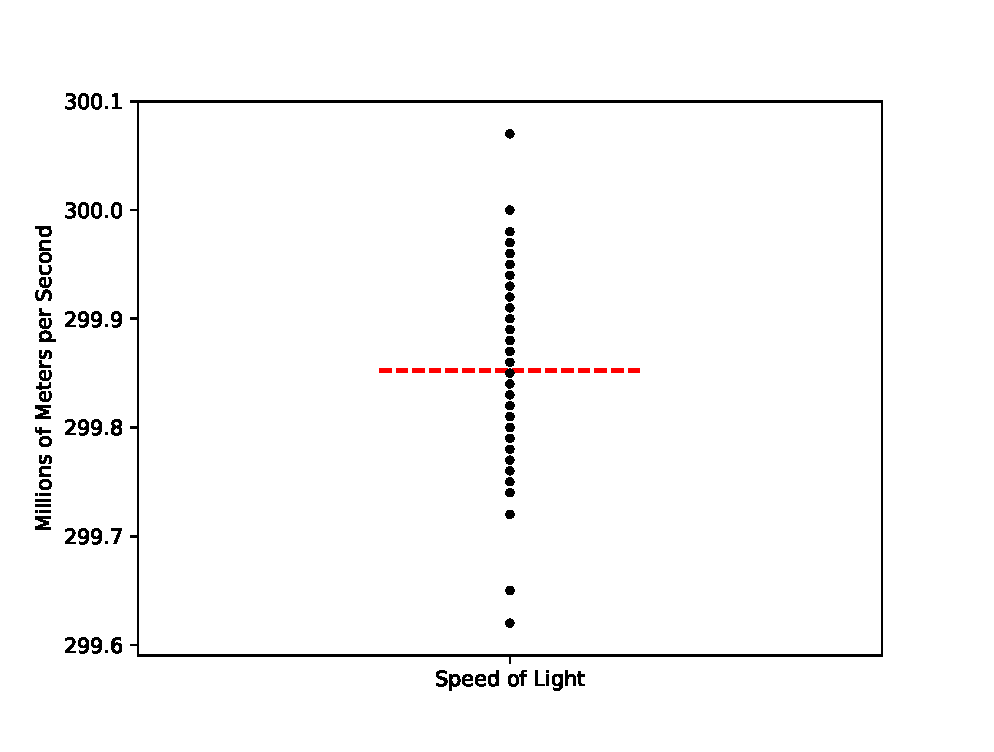
\includegraphics[width=0.85\textwidth]{./images/michelson_scatter}

  \caption{Albert Michelson's 1880 speed-of-light measurements. The mean is
    appropriate as a nominal value. The exact value is plotted for comparison.
    Visually, Michelson's mean value is `close' to the true value, though this
    begs the question `how close is close?' We can make the notion of
    `closeness' more precise by considering the variability of the data.}
  \label{fig:michelson-mean}
\end{figure}

\marginnote{Somewhat cheekily, we can note that $c = 299,792,458 m/s$ is
  \emph{exact}, as the meter is \emph{defined} in terms of the speed of
  light.\cite{thompson2008}}

While the mean is a sensible measure of central tendency, it does have some
weaknesses. We will illustrate these by contrasting against another measure of
central tendency.

\bigskip
The \emph{median}\marginnote{\underline{Concept:} The \emph{sample median} is
  the middle value of a dataset. It is a robust measure of central tendency.} is
the `middle' value of a dataset, most easily described through an example.
Suppose our data is given by $\{5, 3, 6, -1, 4\}$. We find the median by
ordering the data $\{-1, 3, 4, 5, 6\}$ and selecting the middle number; in this
case $4$. In the case where we have an even number of data points, we average
the middle two values.\footnote{e.g. $\{5, 3, 6, -1\}$ yields $\f12(3+5) = 4$}

More generally, we can understand the median in terms of \emph{order
  statistics}, which are simply the ordered values of a dataset. Given our data
$X_i$, the order statistics are defined by

\begin{equation} \label{eq:def-order}
  X_{(1)} \leq X_{(2)} \leq \dots \leq X_{(n-1)} \leq X_{(n)}.
\end{equation}

\noindent The median is then given by $X_{(n/2)}$, which is simply notation for
the middle value. A definition which automatically handles the $n$ odd case is
given by

\begin{equation} \label{eq:def-sample-median}
  \tilde{X} = \f12\left(X_{(\floor{n/2})} + X_{(\ceil{n/2})}\right),
\end{equation}

\noindent where $\floor{\cdot}, \ceil{\cdot}$ define the floor and ceiling
functions. Figure \ref{fig:income-median} provides an example usage of the
median using data from the US Census Bureau. A small number of very large values
(sometimes called \emph{outliers}) can significantly impact the mean. In these
cases, the median can be a better measure of central tendency.

\begin{figure}[!ht]
  \centering
  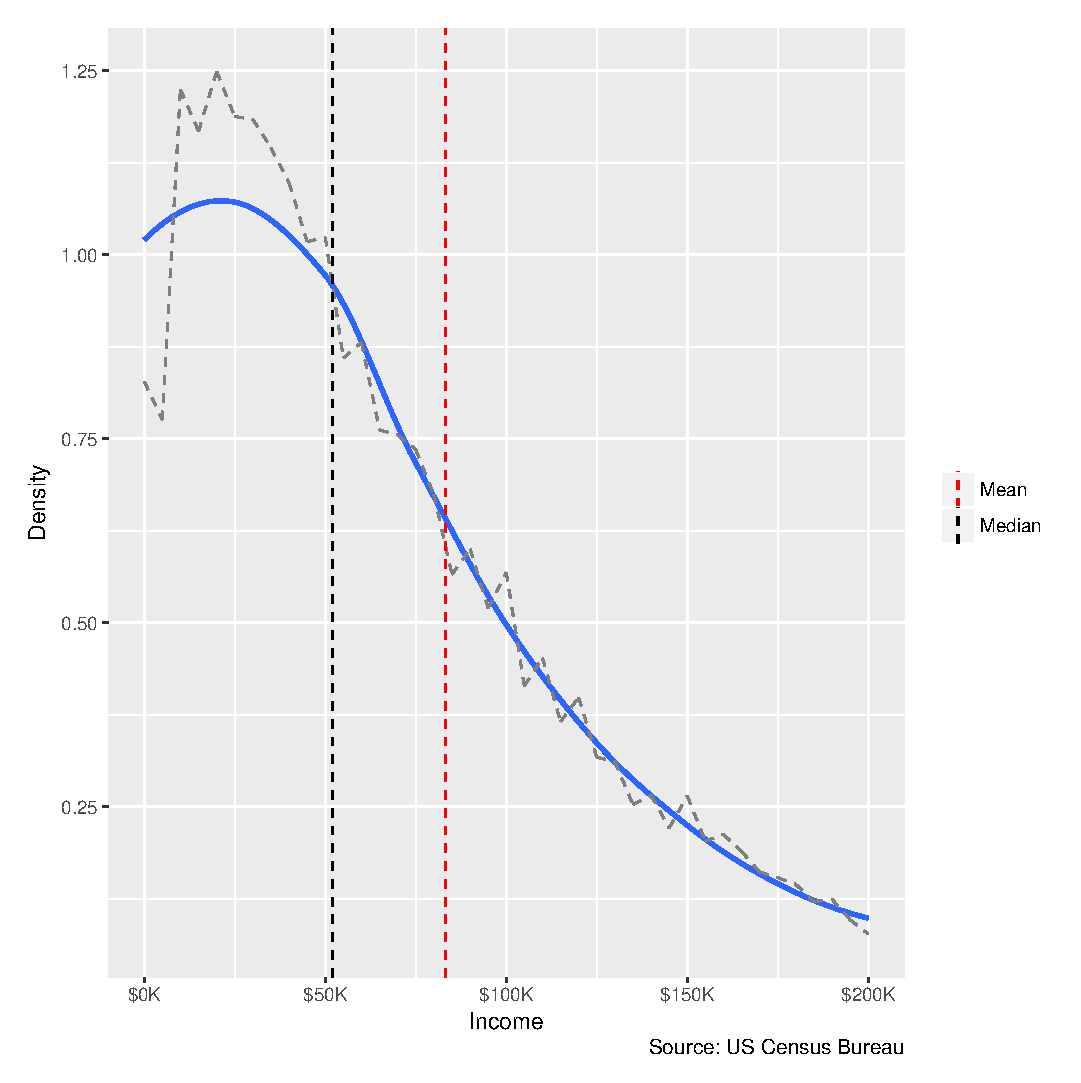
\includegraphics[width=0.85\textwidth]{./images/income}

  \caption{Distribution of sampled household incomes in the US, circa 2016.
    We'll cover density plots a bit later; but for now note that a higher
    density corresponds to a larger number of instances of that income. Notice
    that mean is pulled considerably towards higher incomes, despite the
    preponderance of lower incomes. The median is less affected by a small
    number of large values -- it is often used as a nominal value for income.
    The fact that the mean and median do \emph{not} agree here is telling -- it
    signals that something worth noting is happening in the data.}
  \label{fig:income-median}
\end{figure}

\textbf{Spread} is another apt term for a property of data. The spread is
synonymous with the variability of the data. If our data are thought to be
corrupted measurements of a true value, then spread can be thought of as the
inverse of precision. Similar to central tendency, we will introduce two notions
of spread.\footnote{In fact, in statistics lingo, \emph{precision} is inverse
  variance.}

The \emph{standard deviation}\marginnote{\underline{Concept:} The \emph{sample
    variance} is the mean-squared distance of the data from its mean. The
  \emph{sample standard deviation} is its square root. Both are measures of
  spread.} is a common measure of spread. It is defined via

\begin{equation} \label{eq:def-sample-sd}
  S = \sqrt{\frac{1}{n-1}\sum_{i=1}^n (X_i - \overline{X})^2}.
\end{equation}

Note that we must first compute the sample mean $\overline{X}$ before we can
compute $S$. Somewhat mysteriously, the denominator for $S$ is $n-1$, not $n$.
This is a subtle point that will have to wait until we introduce distributions.
For now, it will suffice to say that for small $n$, this factor\footnote{called
  the \emph{Bessel correction}} is necessary to ensure an accurate
estimate.\footnote{A bit more detail: Using the sample mean $\overline{X}$
  within $S$ causes us to loose a \emph{degree of freedom} -- a notion of
  information available from the data. We account for this `double use' of
  information through the Bessel correction.}

One may use the standard deviation to construct ranges, rather than single
values.\marginnote{A wider interval is less trustworthy than a narrow one; there
  are more true values that are compatible with the available data. One can use
  a confidence interval to draw more robust conclusions; if the entire interval
  is compatible with some conclusion -- if the interval itself falls within some
  acceptable range -- then this enables one to draw a more robust conclusion.} A
common construction is a \emph{confidence interval}, which is a simple idea with
some subtle points. Essentially, if there exists a true value -- like $Y$ --
then a confidence interval will include that value at some known
\emph{confidence level}, often $95\%$ or $99\%$. An interval gives more
information than a mean alone; in addition to location, it conveys the quality
of an estimate, based on its width.

Figure \ref{fig:michelson-ci} depicts a $95\%$ confidence interval for the speed
of light, based on Michelson's 1879 data. Note that this interval includes the
true value, and gives an accurate sense of the spread of the data.

\begin{figure}[!ht]
  \centering
  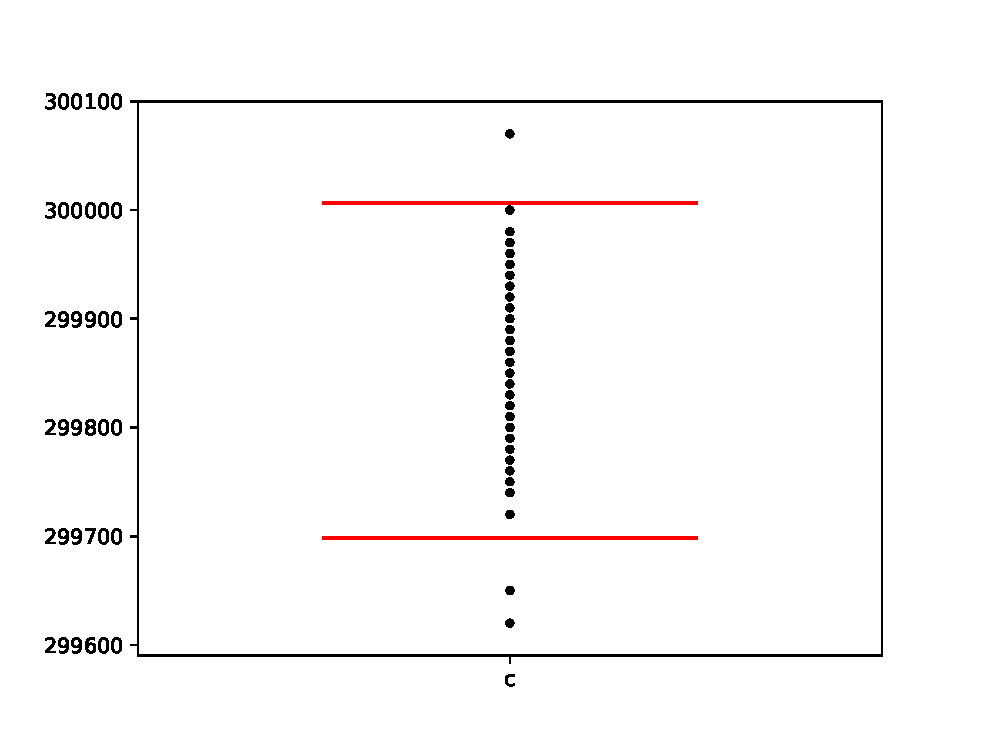
\includegraphics[width=0.85\textwidth]{./images/michelson_ci}

  \caption{Albert Michelson's 1880 speed-of-light measurements. The standard
    deviation is used to construct a confidence interval around the sample mean,
    which here includes the true speed of light. We will introduce the notion of
    \emph{confidence intervals} later when we discuss distributions.}
  \label{fig:michelson-ci}
\end{figure}

The \emph{interquartile range}\marginnote{\underline{Concept:} The \emph{sample
    interquartile range} is the distance between the sample quartiles. It a
  robust measure of spread.} is to the standard deviation as the median is to
the mean. It is a robust measure of spread, and as its name implies it involes
the difference between \emph{quartiles} (the quarter-quantiles) of the data. We
can compute the interquartile range via

\begin{equation} \label{eq:iqr-sample}
  \text{IQR} = Q_3 - Q_1,
\end{equation}

\noindent where $Q_1$ is the median of the lower $\floor{N/2}$ of the data, and
$Q_3$ is the median of the upper fraction.[CITATION NEEDED] The mean was
susceptible to outliers; since the variance is essentially a mean of
squared-differences, the standard deviation is similarly vulnerable to outliers.

(Boxplot example)

\textbf{Skepticism} is vitally important when analyzing data.

\emph{Approaches} are important, and when analyzing data, one should employ
multiple methods to compare their results. Tukey\cite{tukey1979robust}
stated this quite directly when he wrote

\begin{quote}
It is perfectly proper to use both classical and robust/resistant methods
routinely, and only worry when they differ enough to matter. BUT when they
differ, you should think HARD.
\end{quote}

This is why we covered both classical (mean, standard deviation) and robust
(median, iqr) summaries -- in practice, you should use both.

\emph{Outliers}

\emph{Errors}

\begin{figure}[!ht]
  \centering
  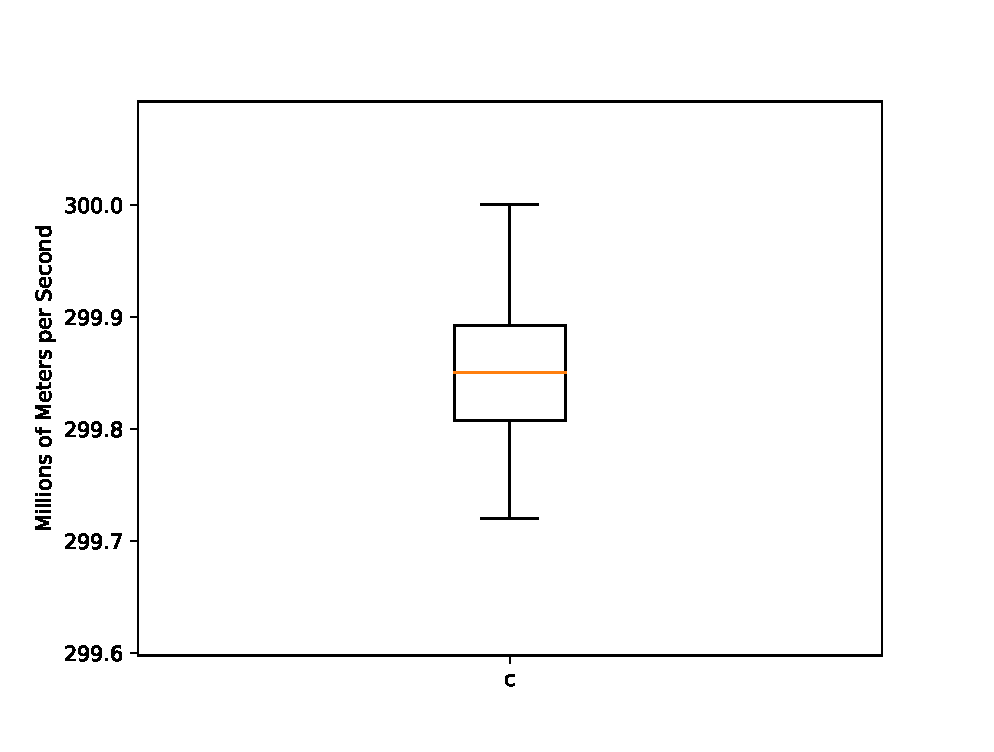
\includegraphics[width=0.85\textwidth]{./images/michelson_boxplot}

  \caption{Albert Michelson's 1880 speed-of-light measurements. The data are
    presented as a boxplot, which highlights a number of potential outliers.}
\end{figure}

\subsection{Distributions}
%% -------------------------

\section{Models}
%% --------------------------------------------------

\section{Questions}
%% --------------------------------------------------


\end{document}
